\documentclass{winslabreport}
\reporttitle{Privacy-Preserving Compution of Total Number of Spanning Tress}
\coursename{CENG519 Network Security}
\courseterm{2021-2022 Spring}
\reportpurpose{Term Project Report}
\authorname{Özgür Aslan}
\studentnumber{e2236958}
\useremail{aslan.ozgur@metu.edu.tr}
\program{Computer Engineering}




\usepackage{algorithmicx,algpseudocode}
\algnewcommand\Input{\item[\textbf{Input:}]}%
\algnewcommand\Output{\item[\textbf{Output:}]}%
\newcommand\tab[1][1cm]{\hspace*{#1}}

\algnewcommand{\Implement}[2]{\item[\textbf{Implements:}] #1 \textbf{Instance}: #2}%
\algnewcommand{\Use}[2]{\item[\textbf{Uses:}] #1 \textbf{Instance}: #2}%
\algnewcommand{\Trigger}[1]{\Statex{\textbf{Trigger:} (#1)}}%
\algnewcommand{\Functions}[1]{\item[\textbf{Functions:}] #1}%
\algnewcommand{\Need}[1]{\item[\textbf{Needs:}] #1}%
\algnewcommand{\Event}[2]{\Statex \item[\textbf{#1:}](#2) \textbf{do}}%
\algnewcommand{\Trig}[3]{\State \textbf{Trigger}  #1.#2 (#3) }%
\algnewcommand{\Foreach}[2]{\State \textbf{for each} #2 \textbf{in} #1 \textbf{do}}%

\def\true{\textbf{T}}
\def\false{\textbf{F}}


\begin{document}
\restoregeometry
\maketitle

\summary
This report explains the secure computation of the total number of spanning trees using homomorphic encryption. The algorithm implemented is Kirchhoff's Matrix Tree Theorem for connected graphs, utilizing the matrix multiplications of the laplacian matrix's lower and upper triangular decomposition. The computation is iterative, where a server and a client communicate back and forth. The server does the calculations on encrypted data. The client performs only the division operation on plain text. The code is implemented with python using the Microsoft Eva compiler for the Microsoft Seal library. The implementation is tested using connected Watts–Strogatz graphs of varying node sizes (between 4 and 64). Extensive analysis of the compilation, execution, key generation, encryption, decryption times, and implementation correctness is shown. Moreover, the effectiveness of using matrix multiplications instead of a loop-based method is discussed for execution times and memory usage. To sum up, this report presents a time and memory-efficient privacy-preserving implementation of Kirchhoff's Matrix Tree Theorem for connected graphs.

\tableofcontents
\listoffigures
%\listoftables
\body

\section{Introduction}
Starting with a real-world example from \cite{MSTExamp}, think of a telecommunication company that wants to layout new fiber-optic cables to some neighborhoods. Each neighborhood will have distinct cabling processes. For each neighborhood, the company has a graph depicting the routes for cable layout as edges and houses that will connect to the new cables as nodes. The telecommunication company wants to finish the layout process as fast as possible using the least resources. But the neighborhoods can have different reasons to prevent or delay the process. So, the company decided to analyze how many different ways efficient cabling can be done and start with the neighborhood that has the most different ways. 

In this example, the company using the graphs of neighborhoods should compute the total number of minimum spanning trees. However, the graphs of the neighborhoods contain critical information that unwanted third parties should not seize. Therefore, the graphs must be encrypted, and any operation on those graphs should be done on the encrypted data. This way, the company can share the information with trusted parties, and the company can outsource computations without a worry. From this extended example, one can understand the importance of graph analytic algorithms, such as computing the total spanning trees and the algorithms' encryption.

Luckily with the advancement of homomorphic encryption, we can do computations on encrypted data and then decrypt to get the results as we did the operations on the plain-text data. I implemented Kirchhoff's matrix tree theorem using the Microsoft Seal library and Microsoft Eva Compiler for Seal. 

Implemention of this algorithm contains many components. Given the graph's adjacency matrix, the first step is to compute the Laplacian of the adjacency matrix. Then calculating any cofactor of the Laplacian matrix will give the total number of spanning trees of the graph. However, calculating the cofactor means computing the determinant. Computing determinant takes in most of the algorithms O($n^3$) times. But Gaussian elimination-based algorithms can be complex to implement with homomorphic encryption frameworks like Seal. Therefore, I have chosen a LU decomposition-based algorithm for computing the determinant. This way, after the decomposition, the determinant is equal to the multiplication of diagonal elements of the upper triangular matrix. The only thing left is to choose a simple decomposition algorithm that can be implemented with Seal. In that aspect, I have selected the Doolittle Algorithm for LU decomposition, which is an iterative algorithm to compute the decomposition. 

The most crucial element of the Doolittle algorithm is that it can be implemented as iterative matrix multiplications and updates of the matrices. Due to interest in doing neural network-based operations in an encrypted fashion using homomorphic encryption, there is a lot of research on efficient homomorphic matrix operations. \cite{10.1145/3243734.3243837, https://doi.org/10.48550/arxiv.2201.12577, Mishra2018FastSM} And I have chosen the work by Jiang et al. \cite{10.1145/3243734.3243837} for matrix multiplication operations as the test results and comparisons with a loop-based Dolittle Algorithm show the effectiveness of the implemented version.


\section{Background and Related Work}

\subsection{Background}

%This section (1 page at most for background) provides the background information needed for the rest of your report to be understood. 

As mentioned in the Introduction, the main components of the algorithm are:
Computing the Laplacian Matrix
Computing the cofactor of Laplacian using LU Decomposition
Homomorphic encryption of these steps using Microsoft SEAL
In this section, necessary background information about these components is given.

As mentioned in the Introduction, the main components of the algorithm are:
\begin{itemize}
    \item Computing the Laplacian Matrix
    \item Computing the cofactor of Laplacian using LU Decomposition
    \item Homomorphic encryption of these steps using Microsoft SEAL
\end{itemize}
In this section, necessary background information about these components is given.
\subsubsection{Homomorphic Encryption}
Most encryption algorithms are used to preserve data security while storing or transferring the data. However, with the advancements in cloud computing, many people use cloud resources to process the data, which cannot be done securely with the classical encryption algorithms.
The encrypted data is decrypted before computation, then the calculation is done on the plain-text data, and finally, the result is encrypted and sent back. The decryption of the data in the cloud causes security concerns.
With homomorphic encryption, the computation is done on the encrypted data. Therefore, there is no need to decrypt the data in the cloud, so the data stays secure.
In this implementation, due to working with floating numbers, CKKS scheme is used. CKKS provides approximate floating point arithmetic on cipher-text, with addition, multiplication and rotation (shifting) of cipher-text. 
\subsubsection{Laplacian Matrix}
The Laplacian matrix is another representation of graphs similar to the adjacency matrix. The Laplacian matrix is the discrete approximation of the continuous Laplacian operator on graphs. It encodes beneficial graph properties, which are used in many machine learning-based algorithms. One can compute it from the adjacency matrix as:
\begin{equation}
    L = D - A,
\end{equation}
where $L$ is the Laplacian Matrix, the $A$ is the Adjacency Matrix and $D$ is the Degree Matrix. Degree Matrix is a diagonal matrix, containing number of neighbours for each node.

\subsubsection{LU Decomposition}
LU Decomposition is the factorization of a matrix to a multiplication of two matrices. One of the matrices is an upper triangular, and the other is a lower triangular hence the name. It is used for efficiently solving linear equations, matrix inversion, and computing the determinant. In the determinant case, the computation of the determinant reduces to the multiplication of diagonal elements of the upper triangular matrix.

\subsection{Related Work}

In this section, two principal algorithms used for computing the total number of spanning trees are introduced. The first algorithm is called Doolittle Algorithm for LU Decomposition. As mentioned in the Background section, factorization makes the determinant easier and keeps the complexity of the computation to $O(n^3)$. The Doolittle Algorithm is an iterative algorithm to compute decomposition:\cite{doolittle}:
\begin{equation}
\label{eqn:dl_it}
\begin{split}
    i &= 0 \xrightarrow[]{\forall j} U_{ij} = A_{ij}, \\ 
    i &> 0 \xrightarrow[]{\forall j} U_{ij} = A_{ij} - \sum_{k=0}^{i-1} L_{ik}U_{kj}, \\
    j &= 0 \xrightarrow[]{\forall i} L_{ij} = \frac{A_{ij}}{U_{jj}}, \\
    j &> 0 \xrightarrow[]{\forall i} L_{ij} = \frac{A_{ij}- \sum_{k=0}^{j-1} L_{ik}U_{kj}}{U_{jj}}. 
\end{split}
\end{equation}
That is, starting with the first row of the upper triangular and first column of the lower triangular matrix, at each iteration the rows of upper triangular and columns of the lower triangular matrices are computed.
In these computations, the only non-trivial computation with homomorphic encryption is the division. There are works \cite{10.1007/978-3-319-70694-8_15} that introduce approximation of inverse function. However, using a these approximations with the other computations makes the overall architecture complex. 
The second algorithm important for the implementation is efficient matrix multiplications with homomorphic encryption \cite{10.1145/3243734.3243837}. Matrix multiplications are used for computing the upper and lower triangular matrices. The reasons are discussed in the next section.


\section{Main Contributions}

\subsection{Client-Server Architecture}
Since the computation of inverse function with Homomorphic Encryption is complex, a server-client architecture is implemented. Meaning that, in an iterative fashion, the server does the computations on the encrypted data, sends it to the client, client decrypts and does the division operation and updates the lower triangular matrix. If the computations are not finished, client encrypts the data and sends it back to server for next computation. The number of iterations are both known by the client and the server, but only client updates it.

At the start, the data send to the server as input is the graph's adjacency matrix. The adjacency matrix is encoded as a plain-text such that rows of the adjacency matrix is concatenated and a vector is obtained. The plain-text is encrypted by the client and send to the server. At the zeroth iteration, the laplacian matrix is computed and the first row and first column of the upper and lower triangular matrices are filled. The server returns the concatenation of the laplacian, upper triangular and lower triangular matrices to the client. Client decrypts the return, updates the iteration, and using the iteration variable computes the inverse of the necessary upper triangular matrix element and updates the lower triangular matrix with it. After the computations by the client, client encrypts the concatenated matrices and sends it to server. After the zeroth iteration, the server computes the matrix multiplication of the lower and upper triangular matrices using the methods introduced in \cite{10.1145/3243734.3243837}. Then using the result of the multiplication, the graph laplacian and masks computed using the iteration variable, server updates the matrices. The number of iterations are the number of nodes n. After the last iteration, the client computes the total number of spanning trees using the upper triangular matrix.

%\begin{algorithm}
%	\def\algorithmlabel{Client}
%    \caption{\algorithmlabel\ process}
%    \label{alg:client}
%    \begin{algorithmic}[1]
%    	\Implement {\algorithmlabel}{cl} 
%    	\Use {SEAL} {seal} 
%    	\Functions{PrepareInput, UpdateInputs, UpdateIteration}
%	    \Need {Adjacency Matrix}
%
%        \Event {PrepareInput}{Adjacency Matrix}
%            \State $plaintext \gets vector$
%            \Foreach {$Adjacency Matrix$}{$row$} 
%                \State $plaintext.extend(row)$
%    \end{algorithmic}
%\end{algorithm}

\subsection{Computing Laplacian Matrix}
To compute the Laplacian Matrix, first the Degree Matrix is computed. Since the adjacency matrix is encoded as a vector, it is relatively easy to compute the Degree Matrix. For an Adjacency Matrix with n nodes, each row can be summed using n left shifts and adding the shifted vector to original vector. After the summations, using plain-text mask vector and right shifts a diagonal degree matrix can be obtained. Subtracting the adjacency matrix from the diagonal degree matrix gives the Laplacian matrix.
\subsection{Computing LU Decomposition with Matrix Multiplication}
As shown in algorithm \ref{eqn:dl_it}, the classical way of computing Doolittle Algorithm is iterative updates. In the first implementation (tagged as \href{https://github.com/ozgraslan/CENG519-Project/tree/milestone3}{milestone3} in the github repository), the iterative version is implemented. However, due to memory issues discussed in \ref{res_dis}, a matrix multiplication based version (tagged as \href{https://github.com/ozgraslan/CENG519-Project/tree/milestone3.4}{milestone3.4}) is implemented. Using a matrix multiplication based version comes from the observation that at iteration i, the $i^{th}$ row and column of the multiplication of the lower (the columns until the $i^{th}$ column is filled and the other columns are zero) and the upper triangular (the rows until the $i^{th}$ row is filled, the other rows are zero) matrices gives the $i^{th}$ row for the upper triangular matrix, and the subtraction term for the $i^{th}$ column of the lower triangular matrix respectively. 

\section{Results and Discussion}
\label{res_dis}
\subsection{Methodology}
All the experiments presented in the paper is done using python 3.8.10 and the main libraries used for implementation are:
\begin{itemize}
    \item Microsoft SEAL 3.6.4 
    \item Microsoft Eva 1.0.1
    \item Numpy 1.22.3
    \item Networkx 2.7.1
\end{itemize}
The hardware used in the experiments is Intel i9-9900K with 32 GB ram. The experiments are run on 1 core only.

The graphs used in the experiments are connected Watts-Strogatz graphs. The number of neighbours for each node is 3. And the connections are reversed with probability 0.5.

For the experiments the node sizes between 4-60 are used. For each node size, 50 experiments are done.
\subsection{Results}
In this section the results of the matrix-based implementation is presented. Since the algorithm is implemented as iterations between a client and a server, sumation of all iterations are presented. Moreover, the correctness of the algorithm is compared against a plaintext based algorithm (for which networkx library is used), and since CKKS is an aproximate scheme, the implemented algorithm is also run on plaintext data and it is compared to the encrypyted version.
\begin{figure}[H]
	\centering
	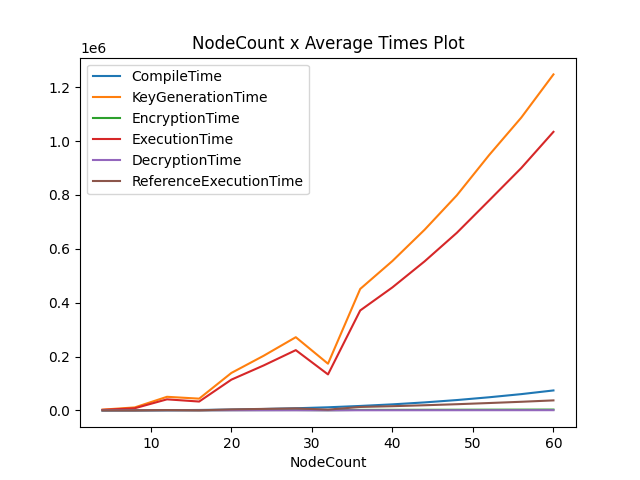
\includegraphics[width=.45\textwidth]{figure/NodeCount x Average Times.png}
	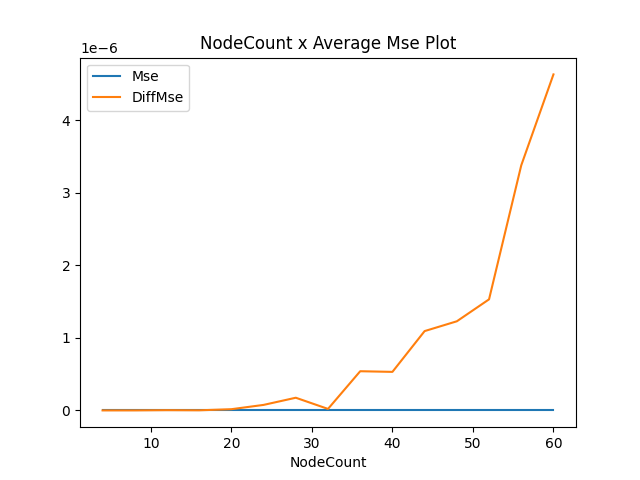
\includegraphics[width=.45\textwidth]{figure/NodeCount x Average Mse.png}
	\caption{The figure on the left shows the summed run times and the figure on the right shows the MSE of the implemented algorithm with an implementation from another library (DiffMse) and MSE of the CKKS approximation and plaintext versions (Mse)}
\end{figure}

From these figures, it can be seen that with the increasing number of nodes the execution times grows exponentially. There are two main reasons for this growth. The first reason is that the number of iterations is the number of nodes. So there are more iterations and the total execution time increases. The second reason which I think is the main reason, the size of the adjacency matrix increases with the node size, therefore the matrix operations take more time. Below figure explains this behaviour.

\begin{figure}[H]
	\centering
	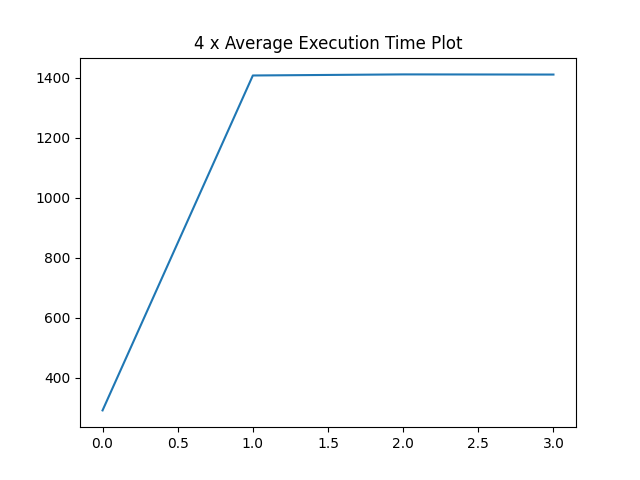
\includegraphics[width=.45\textwidth]{figure/4 x Average Execution Time.png}
	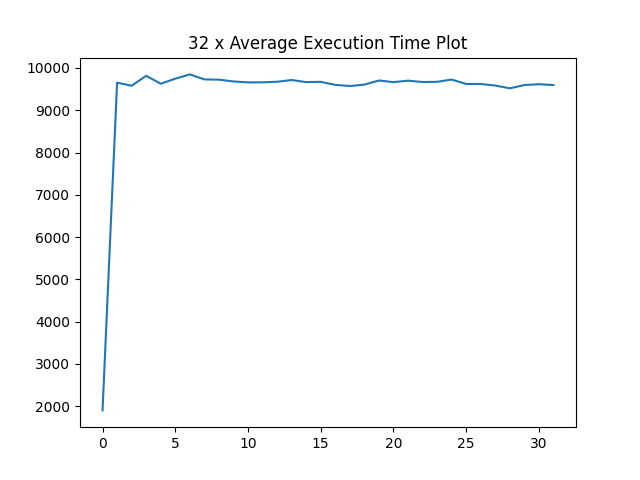
\includegraphics[width=.45\textwidth]{figure/32 x Average Execution Time.png}
	\caption{Two figures (4 Nodes x 32 Nodes) for comparing the execution times for each iteration. Y-axis is execution time in ms and X-axis is the iteration number.}
\end{figure}

\subsection{Discussion}
As mentioned before, the first implementation was iteration based, where iteration number is used as the loop variable. And instead of matrix multiplication, matrix mask operations, vector shifts and summations are used. However, due to loop based implementation, at each iteration the Eva Compiler unrolls the loops and create the plain-text masks before they are used. This increases the memory usage after each iteration. Also, this version uses a lot more plain-text mask at each iteration. This version of the implementation resulted in above 32 GB memory usage even for 24 node graphs. This issue is also discussed in \href{https://github.com/microsoft/SEAL/issues/365}{the SEAL Github Repository}, but there seamed no good solution for my implementation.   

The matrix multiplication version, preserves the memory usage in each iteration, since the matrix does not grow between each iteration. Moreover, it simplifies the implementation with more modular code. With this version, even 64 node graphs can be run with 32 GB memory. 

\section{Conclusion}
This report presents a secure matrix-based implementation of computing the total number of spanning trees in a connected graph. The implementation includes an iterative client-server architecture. In which client only computes the reciprocal of specific values and use those values to updates. The server side computes graph laplacian and doolittle LU decoposition algorihtm using matrix multiplications. As mentioned in the discussion, the matrix-based implementation provides stable memory usage throughout the iterations.  

\bibliographystyle{IEEEtran}
\bibliography{references}
\end{document}
